
\begin{figure}
  \centering
  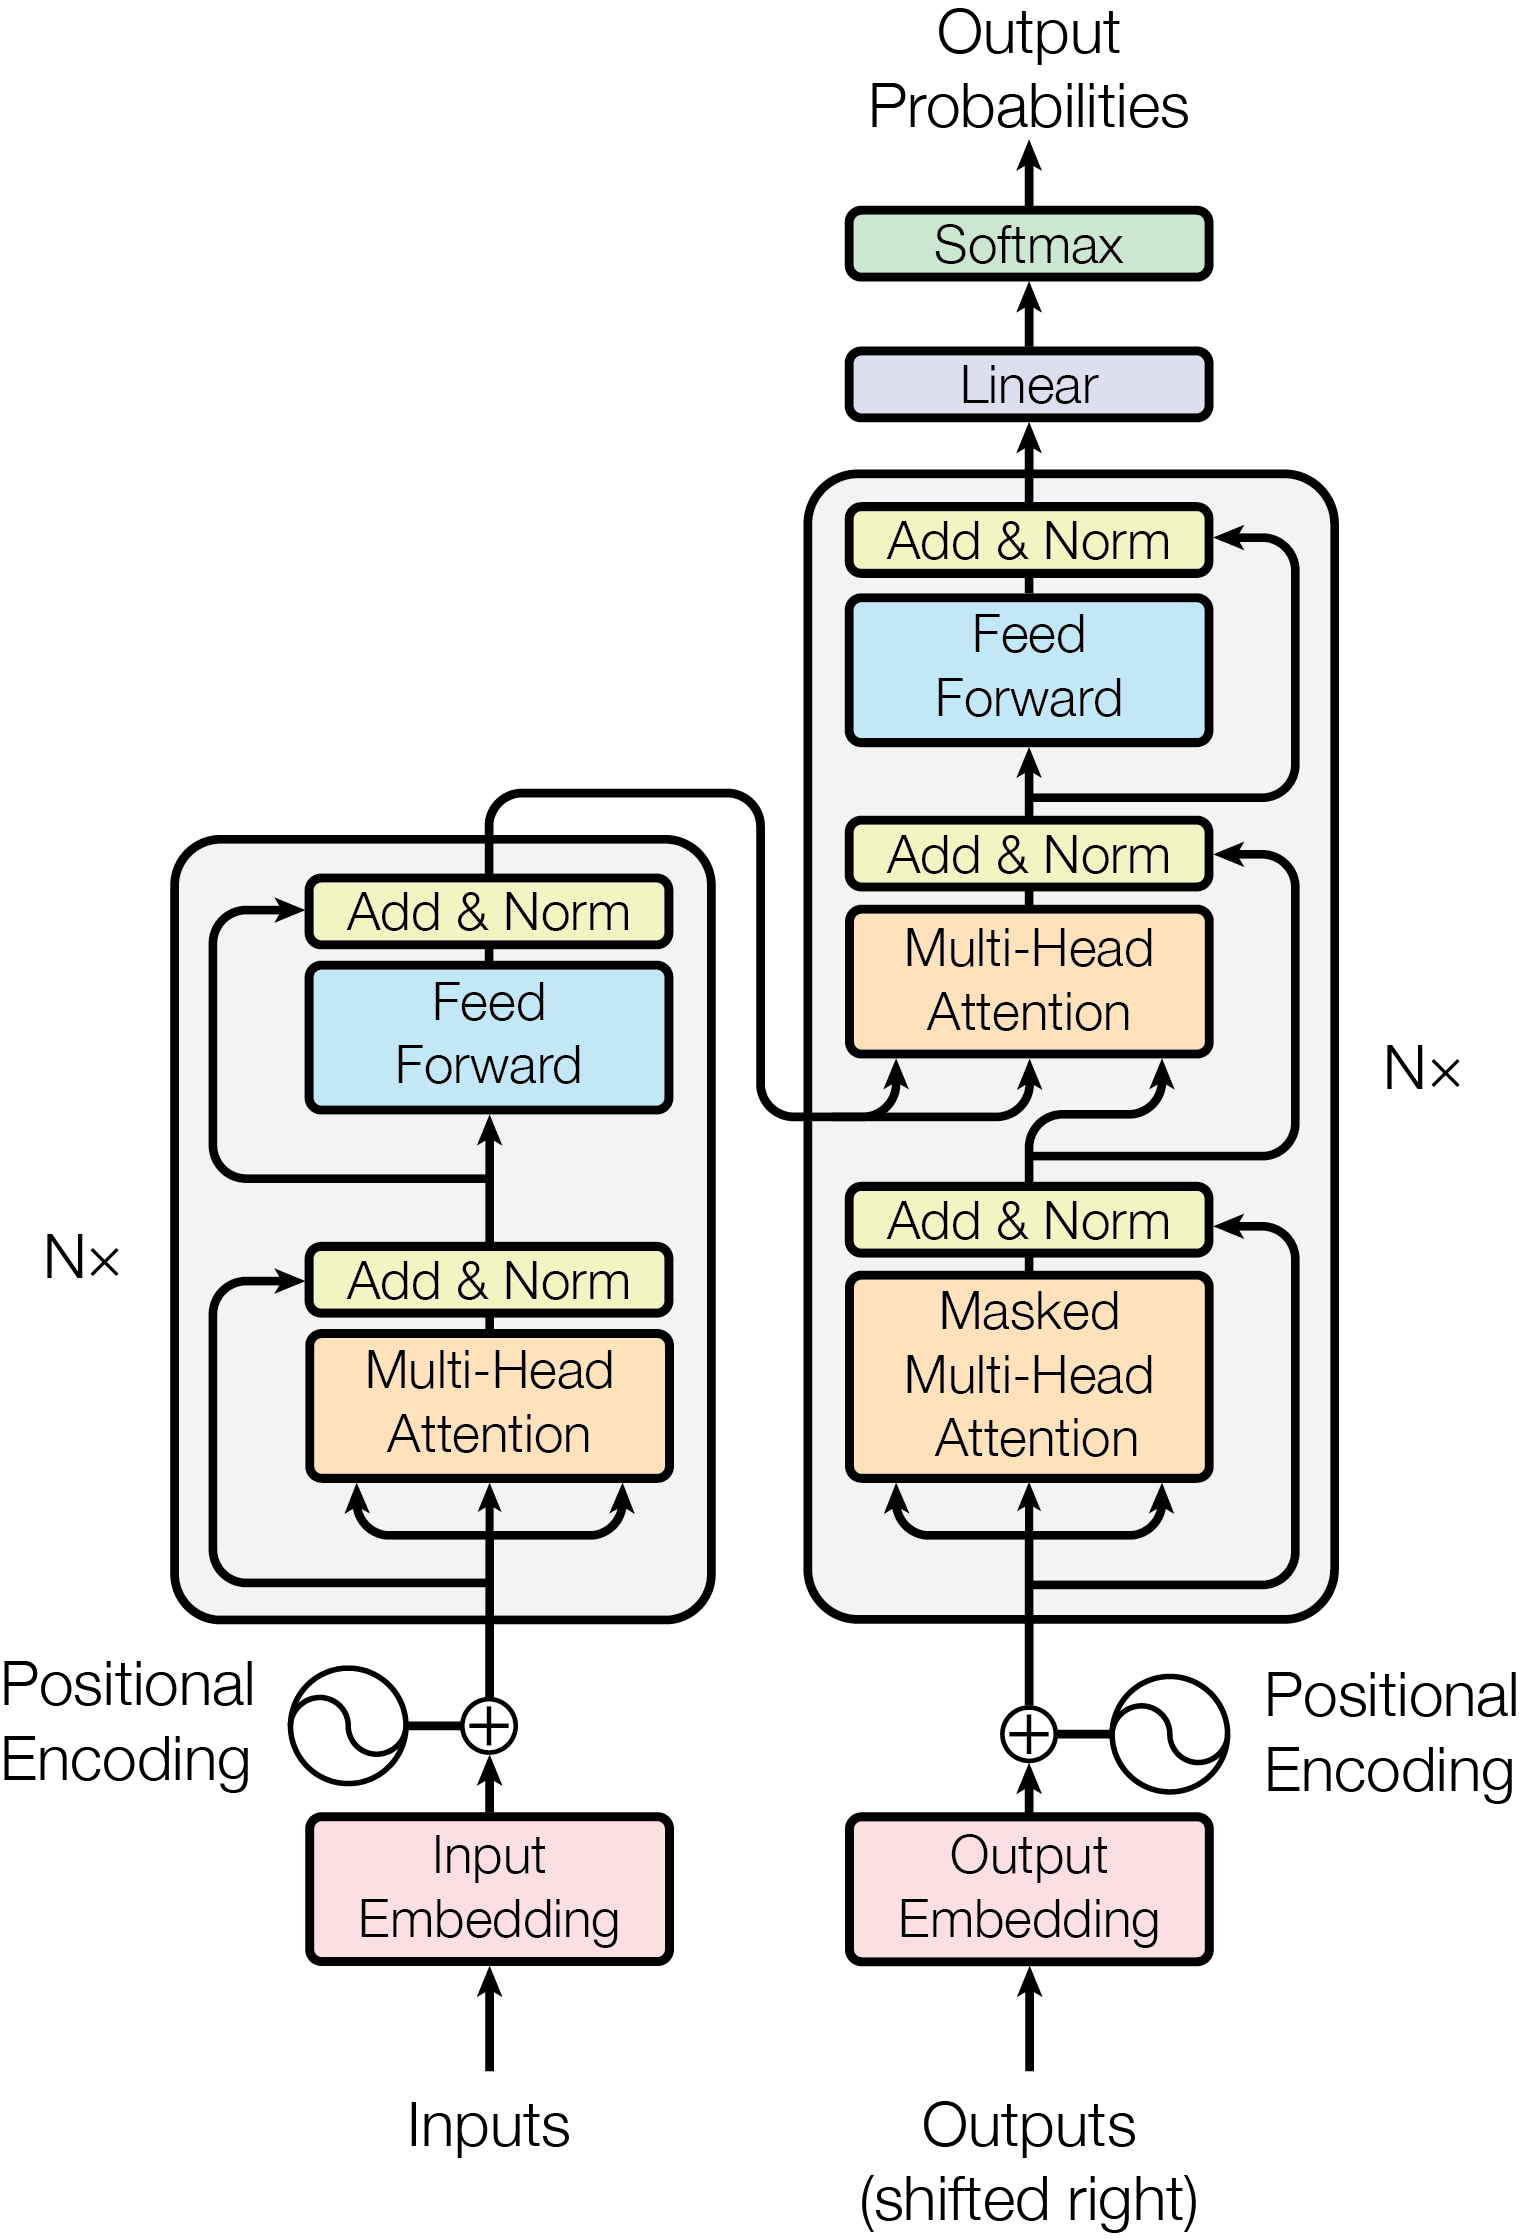
\includegraphics[scale=0.6]{Figures/ModalNet-21}
  \caption{Transformer - 模型结构}
  \label{fig:model-arch}
\end{figure}

% Although the primary workhorse of our model is attention, 
%Our model maintains the encoder-decoder structure that is common to many so-called sequence-to-sequence models \citep{bahdanau2014neural,sutskever14}.  As in all such architectures, the encoder computes a representation of the input sequence, and the decoder consumes these representations along with the output tokens to autoregressively produce the output sequence.  Where, traditionally, the encoder and decoder contain stacks of recurrent or convolutional layers, our encoder and decoder stacks are composed of attention layers and position-wise feed-forward layers (Figure~\ref{fig:model-arch}).  The following sections describe the gross architecture and these particular components in detail.

% Most competitive neural sequence transduction models have an encoder-decoder structure \citep{cho2014learning,bahdanau2014neural,sutskever14}. Here, the encoder maps an input sequence of symbol representations $(x_1, ..., x_n)$ to a sequence of continuous representations $\mathbf{z} = (z_1, ..., z_n)$. Given $\mathbf{z}$, the decoder then generates an output sequence $(y_1,...,y_m)$ of symbols one element at a time. At each step the model is auto-regressive \citep{graves2013generating}, consuming the previously generated symbols as additional input when generating the next.

目前大部分比较热门的神经序列转换模型都是encoder-decoder结构\citep{cho2014learning,bahdanau2014neural,sutskever14}。这里,encoder将输入的一串符号表示$(x_1, ..., x_n)$映射到一串连续表示序列$\mathbf{z} = (z_1, ..., z_n)$. 对于编码得到的$\mathbf{z}$,decoder每次解码生成输出序列$(y_1,...,y_m)$的一个符号,直到生成完整的输出序列。每一步解码都是自回归的\citep{graves2013generating},也就是在生成下一个符号时将先前生成的符号作为附加输入。

% The Transformer follows this overall architecture using stacked self-attention and point-wise, fully connected layers for both the encoder and decoder, shown in the left and right halves of Figure~\ref{fig:model-arch}, respectively.

Transformer在encoder和decoder中都使用了堆叠的self-attention, point-wise和全连接层。encoder和decoder的结构分别如图~\ref{fig:model-arch}的左半部分和右半部分所示。

\subsection{Encoder和Decoder堆}

%\paragraph{Encoder:}The encoder is composed of a stack of $N=6$ identical layers. Each layer has two sub-layers. The first is a multi-head self-attention mechanism, and the second is a simple, position-wise fully connected feed-forward network.   We employ a residual connection \citep{he2016deep} around each of the two sub-layers, followed by layer normalization \cite{layernorm2016}.  That is, the output of each sub-layer is $\mathrm{LayerNorm}(x + \mathrm{Sublayer}(x))$, where $\mathrm{Sublayer}(x)$ is the function implemented by the sub-layer itself.  To facilitate these residual connections, all sub-layers in the model, as well as the embedding layers, produce outputs of dimension $\dmodel=512$.

\paragraph{Encoder:} 编码器由$N=6$个相同的层构成。每层有两个子层。第一个是一个多头的自我注意机制,第二个是一个简单的、位置上的全连接前馈网络。  我们在两个子层的每个周围采用了一个残差连接\citep{he2016deep},然后是层归一化(LayerNorm)\cite{layernorm2016}。 也就是说,每个子层的输出是$\mathrm{LayerNorm}(x + \mathrm{Sublayer}(x))$,其中$\mathrm{Sublayer}(x)$是子层本身实现的函数。为了给这些残差连接便利,模型中的所有子层以及嵌入层都会产生维度为$\dmodel=512$的输出。

%\paragraph{Decoder:}The decoder is also composed of a stack of $N=6$ identical layers.  In addition to the two sub-layers in each encoder layer, the decoder inserts a third sub-layer, which performs multi-head attention over the output of the encoder stack.  Similar to the encoder, we employ residual connections around each of the sub-layers, followed by layer normalization.  We also modify the self-attention sub-layer in the decoder stack to prevent positions from attending to subsequent positions.  This masking, combined with fact that the output embeddings are offset by one position, ensures that the predictions for position $i$ can depend only on the known outputs at positions less than $i$.

\paragraph{Decoder:} 解码器也是由$N=6$的相同层堆栈组成。除了每个编码器层的两个子层之外,解码器还插入了第三种子层,它对编码器堆的输出进行多头注意。与编码器类似,我们在每个子层周围采用残差连接,然后进行层归一化。我们还修改了解码器堆栈中的自注意子层,以防止位置关注后续位置。这种屏蔽,再加上输出嵌入总是偏移一个位置,确保对位置$i$的预测只依赖于小于$i$的位置的已知输出。

% In our model (Figure~\ref{fig:model-arch}), the encoder and decoder are composed of stacks of alternating self-attention layers (for cross-positional communication) and position-wise feed-forward layers (for in-place computation).  In addition, the decoder stack contains encoder-decoder attention layers.  Since attention is agnostic to the distances between words, our model requires a "positional encoding" to be added to the encoder and decoder input. The following sections describe all of these components in detail.

\subsection{注意力机制} \label{sec:attention}
%An attention function can be described as mapping a query and a set of key-value pairs to an output, where the query, keys, values, and output are all vectors.  The output is computed as a weighted sum of the values, where the weight assigned to each value is computed by a compatibility function of the query with the corresponding key.

注意力函数可以被描述为将一个查询(query)和一对键-值(key-value)对映射到一个输出,其中查询(query)、键(key)、值(value)和输出都是向量。输出被计算为值(value)的加权和,其中分配给每个数值的权重是由查询(query)与相应的键(key)的相似函数计算的。

\subsubsection{缩放点积注意力(Scaled Dot-Product Attention)} \label{sec:scaled-dot-prod}

% \begin{figure}
%   \centering
%   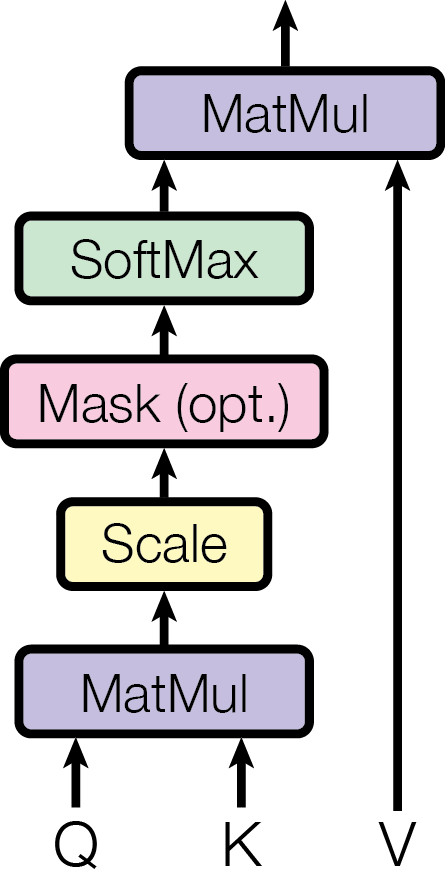
\includegraphics[scale=0.6]{Figures/ModalNet-19}
%   \caption{Scaled Dot-Product Attention.}
%   \label{fig:multi-head-att}
% \end{figure}

%We call our particular attention "Scaled Dot-Product Attention" (Figure~\ref{fig:multi-head-att}).   The input consists of queries and keys of dimension $d_k$, and values of dimension $d_v$.  We compute the dot products of the query with all keys, divide each by $\sqrt{d_k}$, and apply a softmax function to obtain the weights on the values.

我们把我们自己的独特的注意力机制称为 “缩放点积注意力”(Scaled Dot-Product Attention)(Figure~\ref{fig:multi-head-att})。 输入包括查询(query)和维度为$d_k$的键(key),以及维度为$d_v$的值(value)。 我们计算查询(query)与所有键(key)的点积,将每个键除以$\sqrt{d_k}$,并应用softmax函数来获得值(value)的权重。

%In practice, we compute the attention function on a set of queries simultaneously, packed together into a matrix $Q$.   The keys and values are also packed together into matrices $K$ and $V$.  We compute the matrix of outputs as:

在实践中,我们同时计算一组查询(query)的注意力函数,并将其打包成一个矩阵$Q$。键(key)和值(value)也被打包成矩阵$K$和$V$。我们计算输出的矩阵为:

\begin{equation}
   \mathrm{Attention}(Q, K, V) = \mathrm{softmax}\left(\frac{QK^T}{\sqrt{d_k}}\right)V
\end{equation}

%The two most commonly used attention functions are additive attention \citep{bahdanau2014neural}, and dot-product (multiplicative) attention.  Dot-product attention is identical to our algorithm, except for the scaling factor of $\frac{1}{\sqrt{d_k}}$. Additive attention computes the compatibility function using a feed-forward network with a single hidden layer.  While the two are similar in theoretical complexity, dot-product attention is much faster and more space-efficient in practice, since it can be implemented using highly optimized matrix multiplication code.

两种最常用的注意力函数是加法注意力\citep{bahdanau2014neural},和点积(乘法)注意力。 除了$\frac{1}{\sqrt{d_k}}$的比例因子外,点积注意力与我们的算法相同。加法注意力使用具有单个隐藏层的前馈网络来计算兼容性函数。 虽然两者在理论上的计算复杂度相似,但点积式注意力在实践中要快得多,而且空间效率更高,因为它可以用高度优化的矩阵乘法代码来实现。

%We scale the dot products by $1/\sqrt{d_k}$ to limit the magnitude of the dot products, which works well in practice. Otherwise, we found applying the softmax to often result in weights very close to 0 or 1, and hence minuscule gradients.

% Already described in the subsequent section
%When used as part of decoder self-attention, an optional mask function is applied just before the softmax to prevent positions from attending to subsequent positions.   This mask simply sets the logits corresponding to all illegal connections (those outside of the lower triangle) to $-\infty$.

%\paragraph{Comparison to Additive Attention: } We choose dot product attention over additive attention \citep{bahdanau2014neural} since it can be computed using highly optimized matrix multiplication code.  This optimization is particularly important to us, as we employ many attention layers in our model.

%While for small values of $d_k$ the two mechanisms perform similarly, additive attention outperforms dot product attention without scaling for larger values of $d_k$ \citep{DBLP:journals/corr/BritzGLL17}. We suspect that for large values of $d_k$, the dot products grow large in magnitude, pushing the softmax function into regions where it has extremely small gradients  \footnote{To illustrate why the dot products get large, assume that the components of $q$ and $k$ are independent random variables with mean $0$ and variance $1$.  Then their dot product, $q \cdot k = \sum_{i=1}^{d_k} q_ik_i$, has mean $0$ and variance $d_k$.}. To counteract this effect, we scale the dot products by $\frac{1}{\sqrt{d_k}}$.

虽然对于$d_k$比较小的情况,这两种机制的表现相似,但对于$d_k$比较大的情况,加法注意力优于不使用缩放的点积注意力\citep{DBLP:journals/corr/BritzGLL17}。我们怀疑,对于$d_k$比较大的情况,点积的结果的大小受到$d_k$影响而增长,将softmax函数推到它具有极小梯度的区域(译注:梯度消失)。
\footnote{为了说明为什么点积会变大,假设$q$和$k$的组成部分是独立的随机变量,均值为$0$,方差为$1$。 那么它们的点积,$q \cdot k = \sum_{i=1}^{d_k} q_ik_i$,均值为$0$,方差为$d_k$。}
为了抵消这种影响,我们用$\frac{1}{\sqrt{d_k}}$来缩放点积的结果。

%We suspect this to be caused by the dot products growing too large in magnitude to result in useful gradients after applying the softmax function.  To counteract this, we scale the dot product by $1/\sqrt{d_k}$.


\subsubsection{多头注意力机制(Multi-Head Attention)} \label{sec:multihead}

\begin{figure}
\begin{minipage}[t]{0.5\textwidth}
  \centering
  % Scaled Dot-Product Attention \\
  缩放点积注意力 \\
  \vspace{0.5cm}
  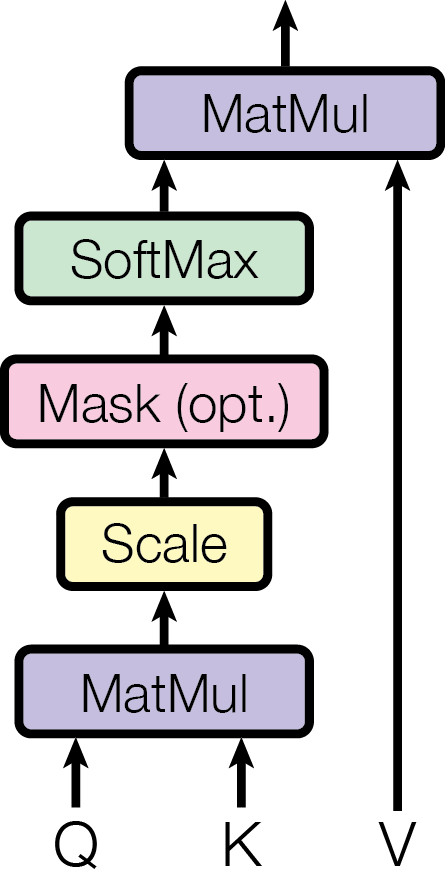
\includegraphics[scale=0.6]{Figures/ModalNet-19}
\end{minipage}
\begin{minipage}[t]{0.5\textwidth}
  \centering 
  %Multi-Head Attention \\
  多头注意力机制 \\
  \vspace{0.1cm}
  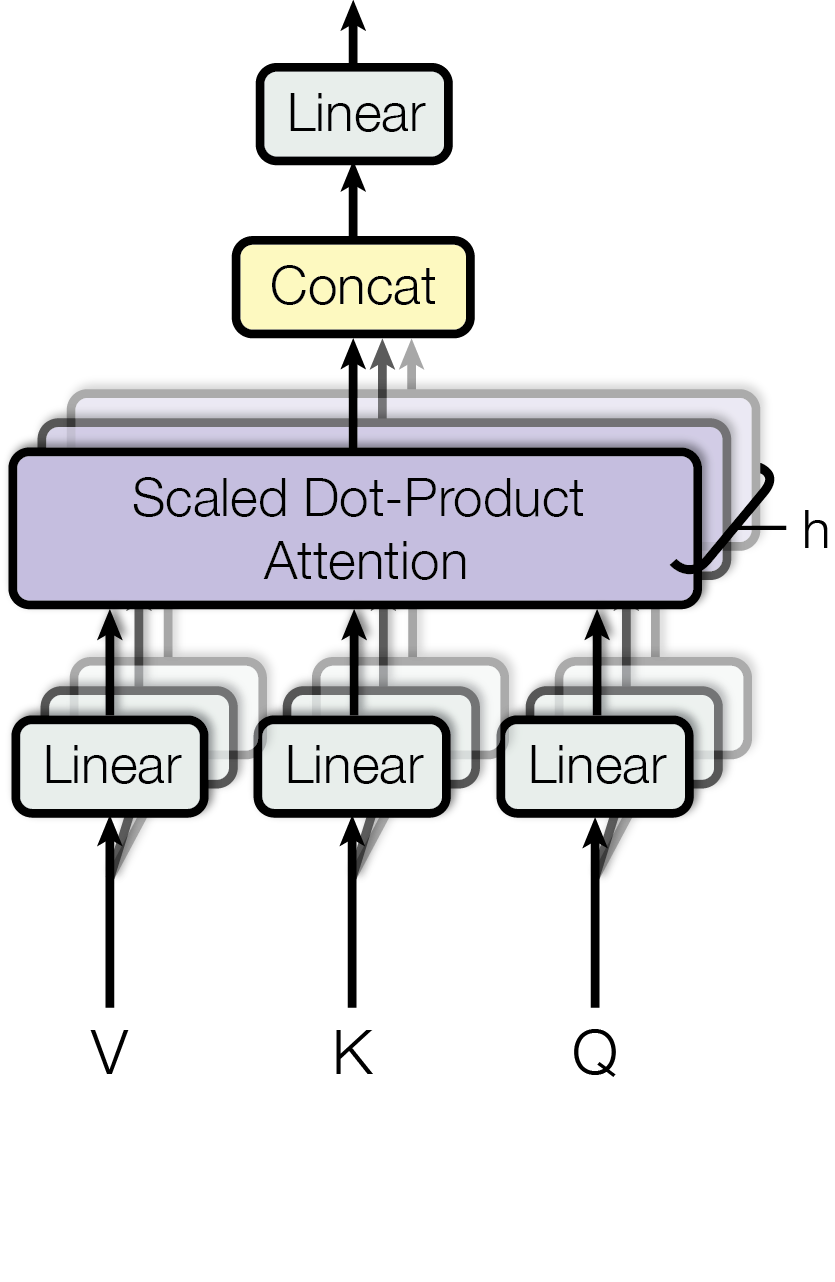
\includegraphics[scale=0.6]{Figures/ModalNet-20}  
\end{minipage}


  % \centering

  %\caption{(left) Scaled Dot-Product Attention. (right) Multi-Head Attention consists of several attention layers running in parallel.} 
  \caption{(左) 缩放点积注意力 (右) 多头注意力机制由几个并行进行的注意力层组成}
  \label{fig:multi-head-att}
\end{figure}

%Instead of performing a single attention function with $\dmodel$-dimensional keys, values and queries, we found it beneficial to linearly project the queries, keys and values $h$ times with different, learned linear projections to $d_k$, $d_k$ and $d_v$ dimensions, respectively.
%On each of these projected versions of queries, keys and values we then perform the attention function in parallel, yielding $d_v$-dimensional output values. These are concatenated and once again projected, resulting in the final values, as depicted in Figure~\ref{fig:multi-head-att}.

我们发现,用不同的、可学习的线性变换将查询、键和值分别变换到$d_k$、$d_k$和$d_v$维度上,而不是用$\dmodel$维度的键、值和查询来执行单一的注意函数。
在每一个通过上述线性变换得到的查询、键和值的基础上,我们再平行地进行注意函数,产生$d_v$维的输出值。这些值被拼接(concatenate)起来,并再次进行线性变换,从而得到最终的值,如图~\ref{fig:multi-head-att}所示。

%Multi-head attention allows the model to jointly attend to information from different representation subspaces at different positions. With a single attention head, averaging inhibits this.
多头注意力机制允许模型在不同的位置上一同关注来自不同表征子空间的信息。在单头注意力的情况下,平均化抑制了这一点。

\begin{align*}
    \mathrm{MultiHead}(Q, K, V) &= \mathrm{Concat}(\mathrm{head_1}, ..., \mathrm{head_h})W^O\\
%    \mathrm{where} \mathrm{head_i} &= \mathrm{Attention}(QW_Q_i^{\dmodel \times d_q}, KW_K_i^{\dmodel \times d_k}, VW^V_i^{\dmodel \times d_v})\\
    \text{where}~\mathrm{head_i} &= \mathrm{Attention}(QW^Q_i, KW^K_i, VW^V_i)\\
\end{align*}

%Where the projections are parameter matrices $W^Q_i \in \mathbb{R}^{\dmodel \times d_k}$, $W^K_i \in \mathbb{R}^{\dmodel \times d_k}$, $W^V_i \in \mathbb{R}^{\dmodel \times d_v}$ and $W^O \in \mathbb{R}^{hd_v \times \dmodel}$.
此处的线性变换是通过参数矩阵提供:$W^Q_i \in \mathbb{R}^{\dmodel \times d_k}$,$W^K_i \in \mathbb{R}^{\dmodel \times d_k}$, $W^V_i \in \mathbb{R}^{\dmodel \times d_v}$ 和 $W^O \in \mathbb{R}^{hd_v \times \dmodel}$.


%find it better (and no more expensive) to have multiple parallel attention layers (each over the full set of positions) with proportionally lower-dimensional keys, values and queries.  We call this "Multi-Head Attention" (Figure~\ref{fig:multi-head-att}).  The keys, values, and queries for each of these parallel attention layers are computed by learned linear transformations of the inputs to the multi-head attention.  We use different linear transformations across different parallel attention layers.  The output of the parallel attention layers are concatenated, and then passed through a final learned linear transformation. 


%In this work we employ $h=8$ parallel attention layers, or heads. For each of these we use $d_k=d_v=\dmodel/h=64$.
%Due to the reduced dimension of each head, the total computational cost is similar to that of single-head attention with full dimensionality.

在这个工作中,我们并行进行$h=8$个注意力层/头,每一个头的维度为$d_k=d_v=\dmodel/h=64$。由于每个头的维度减少,总的计算成本与全维度的单头注意力相似。

%\subsubsection{Applications of Attention in our Model}
\subsubsection{Attention在模型中的应用}

Transformer中以三种不同的方式使用了多头注意力机制:
\begin{itemize}
%  \item In "encoder-decoder attention" layers, the queries come from the previous decoder layer, and the memory keys and values come from the output of the encoder.   This allows every position in the decoder to attend over all positions in the input sequence.  This mimics the typical encoder-decoder attention mechanisms in sequence-to-sequence models such as \citep{wu2016google, bahdanau2014neural,JonasFaceNet2017}.
 \item 在“编码器-解码器注意力”("Encoder-Decoder Attention")层,queries来自先前的解码器层,并且keys和values来自编码器的输出。这使得解码器中的每个位置都能关注到输入序列中的所有位置。这与Seq2Seq模型中的经典的编码器-解码器注意力机制一致\citep{wu2016google, bahdanau2014neural,JonasFaceNet2017}。

 %\item The encoder contains self-attention layers.  In a self-attention layer all of the keys, values and queries come from the same place, in this case, the output of the previous layer in the encoder.   Each position in the encoder can attend to all positions in the previous layer of the encoder.
 \item 编码器中的自注意力层。在自注意力层中,所有的keys、values和queries都来同一个地方,这里都是来自编码器中前一层的输出。编码器中当前层的每个位置都能关注到前一层的所有位置

 %\item Similarly, self-attention layers in the decoder allow each position in the decoder to attend to all positions in the decoder up to and including that position.  We need to prevent leftward information flow in the decoder to preserve the auto-regressive property.  We implement this inside of scaled dot-product attention by masking out (setting to $-\infty$) all values in the input of the softmax which correspond to illegal connections.  See Figure~\ref{fig:multi-head-att}.
 \item 类似的,解码器中的自注意力层允许解码器中的每个位置关注当前解码位置和它前面的所有位置。这里需要屏蔽解码器中向左的信息流以保持自回归属性。具体的实现方式是在缩放后的点积注意分数中,屏蔽(设为负无穷$-\infty$)softmax的输入中所有对应着非法连接的values。见图~\ref{fig:multi-head-att}。

\end{itemize}

\subsection{逐位置前馈网络(Position-wise Feed-Forward Networks)}\label{sec:ffn}

%In addition to attention sub-layers, each of the layers in our encoder and decoder contains a fully connected feed-forward network, which is applied to each position separately and identically.  This consists of two linear transformations with a ReLU activation in between.
除了注意子层之外,我们的编码器和解码器中的每一层都包含一个全连接的前馈网络,该网络分别适用于每个位置,并且完全相同。 这包括两个线性变换,中间有一个ReLU激活。

\begin{equation}
   \mathrm{FFN}(x)=\max(0, xW_1 + b_1) W_2 + b_2
\end{equation}

%While the linear transformations are the same across different positions, they use different parameters from layer to layer. Another way of describing this is as two convolutions with kernel size 1.  The dimensionality of input and output is $\dmodel=512$, and the inner-layer has dimensionality $d_{ff}=2048$.

虽然线性变换(Linear)在不同的位置上是相同的,但它们在不同的层上使用不同的参数。另一种方式是将其作为两个内核大小为1的卷积。其输入和输出的维度为$\dmodel=512$,内层的维度为$d_{ff}=2048$。


%In the appendix, we describe how the position-wise feed-forward network can also be seen as a form of attention.

%from Jakob: The number of operations required for the model to relate signals from two arbitrary input or output positions grows in the distance between positions in input or output, linearly for ConvS2S and logarithmically for ByteNet, making it harder to learn dependencies between these positions \citep{hochreiter2001gradient}. In the transformer this is reduced to a constant number of operations, albeit at the cost of effective resolution caused by averaging attention-weighted positions, an effect we aim to counteract with multi-headed attention.


%Figure~\ref{fig:simple-att} presents a simple attention function, $A$, with a single head, that forms the basis of our multi-head attention. $A$ takes a query key vector $\kq$, matrices of memory keys $\km$ and memory values $\vm$ ,and produces a query value vector $\vq$ as 
%\begin{equation*} \label{eq:attention}
%    A(\kq, \km, \vm) = {\vm}^T (Softmax(\km \kq).
%\end{equation*}
%We linearly transform $\kq,\,\km$, and $\vm$ with learned matrices ${\Wkq \text{,} \, \Wkm}$, and ${\Wvm}$ before calling the attention function, and transform the output query with $\Wvq$ before handing it to the feed forward layer. Each attention layer has it's own set of transformation matrices, which are shared across all query positions. $A$ is applied in parallel for each query position, and is implemented very efficiently as a batch of matrix multiplies. The self-attention and encoder-decoder attention layers use $A$, but with different arguments. For example, in encdoder self-attention, queries in encoder layer $i$ attention to memories in encoder layer $i-1$. To ensure that decoder self-attention layers do not look at future words, we add $- \inf$ to the softmax logits in positions $j+1$ to query length for query position $l$.  

%In simple attention, the query value is a weighted combination of the memory values where the attention weights sum to one. Although this function performs well in practice, the constraint on attention weights can restrict the amount of information that flows from memories to queries because the query cannot focus on multiple memory positions at once, which might be desirable when translating long sequences. \marginpar{@usz, could you think of an example of this ?} We remedy this by maintaining multiple attention heads at each query position that attend to all memory positions in parallel, with a different set of parameters  per attention head $h$. 
%\marginpar{}

\subsection{嵌入和Softmax}
%Similarly to other sequence transduction models, we use learned embeddings to convert the input tokens and output tokens to vectors of dimension $\dmodel$.  We also use the usual learned linear transformation and softmax function to convert the decoder output to predicted next-token probabilities.  In our model, we share the same weight matrix between the two embedding layers and the pre-softmax linear transformation, similar to \citep{press2016using}.   In the embedding layers, we multiply those weights by $\sqrt{\dmodel}$.

与其他序列转换模型类似,我们使用可学习的嵌入将输入标记和输出标记转换为维度为$\dmodel$的向量。我们还使用通常的可学习的线性层(Linear)和softmax函数将解码器输出转换为预测的下一个标记概率。 在我们的模型中,我们在两个嵌入层和pre-softmax(在softmax前面的)线性层之间共享相同的权重矩阵,类似于\citep{press2016using}。在嵌入层中,我们把这些权重乘以$\sqrt{\dmodel}$。

\subsection{Positional Encoding}
%Since our model contains no recurrence and no convolution, in order for the model to make use of the order of the sequence, we must inject some information about the relative or absolute position of the tokens in the sequence.  To this end, we add "positional encodings" to the input embeddings at the bottoms of the encoder and decoder stacks.  The positional encodings have the same dimension $\dmodel$ as the embeddings, so that the two can be summed.   There are many choices of positional encodings, learned and fixed \citep{JonasFaceNet2017}.
由于我们的模型不包含RNN和CNN,为了使模型能够利用序列的顺序,我们必须注入一些关于序列中标记的相对或绝对位置的信息。 为此,我们在编码器和解码器堆栈的底部为输入嵌入添加 “位置编码”(Positional Encoding)。 位置编码与嵌入具有相同的维度$\dmodel$,因此两者可以相加。位置编码有很多选择,有学习的,也有固定的 \citep{JonasFaceNet2017}。


%In this work, we use sine and cosine functions of different frequencies:
在这项工作中,我们使用不同频率的正弦和余弦函数来进行Positional Encoding:

\begin{align*}
    PE_{(pos,2i)} = sin(pos / 10000^{2i/\dmodel}) \\
    PE_{(pos,2i+1)} = cos(pos / 10000^{2i/\dmodel})
\end{align*}

%where $pos$ is the position and $i$ is the dimension.  That is, each dimension of the positional encoding corresponds to a sinusoid.  The wavelengths form a geometric progression from $2\pi$ to $10000 \cdot 2\pi$.  We chose this function because we hypothesized it would allow the model to easily learn to attend by relative positions, since for any fixed offset $k$, $PE_{pos+k}$ can be represented as a linear function of $PE_{pos}$.

其中$pos$是位置,$i$是维度。也就是说,位置编码的每个维度对应于一个正弦波,其波长形成一个几何级数,从$2\pi$到$10000\cdot 2\pi$。我们选择这个函数是因为我们假设它能让模型很容易地学会通过相对位置来进行推理,因为对于任何固定的偏移量$k$,$PE_{pos+k}$可以被表示为$PE_{pos}$的线性函数。

%We also experimented with using learned positional embeddings \citep{JonasFaceNet2017} instead, and found that the two versions produced nearly identical results (see Table~\ref{tab:variations} row (E)).  We chose the sinusoidal version because it may allow the model to extrapolate to sequence lengths longer than the ones encountered during training.

我们也尝试采用可学习的positional embeddings\citep{JonasFaceNet2017}代替上面的方法,然后发现两者得到了几乎一样的结果(见表~\ref{tab:variations}(E)行)。我们选择正弦波版本是因为它可能允许模型推断出比训练期间遇到的序列长度更长的序列。